% ============================================================
%  tikz_fig_bc_trend.tex  ── 上段パネルのみ（スライド1枚目用）
%  【使用例】
%    \begin{frame}{経済成長とトレンド}
%      \input{tikz/tikz_fig_bc_trend}
%    \end{frame}
% ============================================================
\documentclass[tikz, dvipdfmx]{standalone}
\usepackage{tikz}
\usepackage{pgfplots}
\pgfplotsset{compat=1.18}
\usepgfplotslibrary{fillbetween}
\usetikzlibrary{arrows.meta}
\definecolor{gdpblue} {RGB}{30,  90,  180}
\definecolor{trendred}{RGB}{190, 40,  40}
\definecolor{expgreen}{RGB}{200, 230, 200}
\definecolor{recred}  {RGB}{240, 200, 200}

\begin{document}
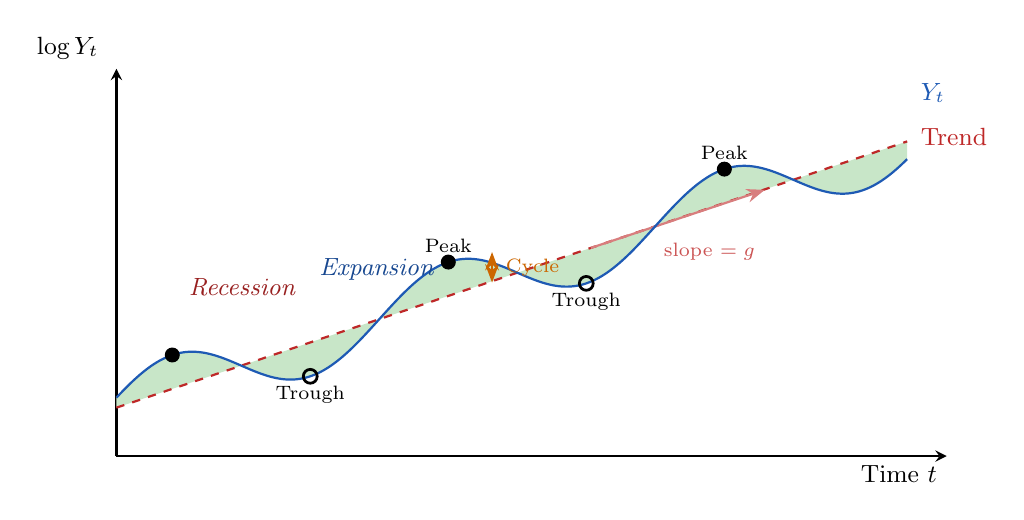
\begin{tikzpicture}
\begin{axis}[
  width  = \linewidth,
  height = 6.5cm,
  xmin = 0, xmax = 10.5,
  ymin = 0.5, ymax = 8.5,
  xtick = \empty, ytick = \empty,
  axis lines      = left,
  axis line style = {thick},
  clip            = false,
  every axis plot/.append style = {smooth},
  font = \small,
  ylabel = {$\log Y_t$},
  ylabel style = {
    rotate = -90,
    at     = {(axis description cs: -0.01, 1.0)},
    anchor = south east,
  },
  xlabel = {Time $t$},
  xlabel style = {
    at     = {(axis description cs: 1.0, 0)},
    anchor = north east,
  },
]
  % ── fill between 用透明パス ─────────────────────────────
  \addplot[draw=none, name path=gdp_path, domain=0:10, samples=300]
    { 0.55*x + 1.5 + 0.7*sin(deg(1.8*x + 0.3)) };
  \addplot[draw=none, name path=trend_path, domain=0:10, samples=2]
    { 0.55*x + 1.5 };

  % ── 拡張（緑）/ 後退（赤）シェーディング ────────────────
  \addplot fill between[
    of = gdp_path and trend_path,
    every even segment/.style = {fill=expgreen},
    every odd  segment/.style = {fill=recred},
  ];

  % ── トレンド線 ───────────────────────────────────────────
  \addplot[trendred, thick, dashed, domain=0:10, samples=2]
    { 0.55*x + 1.5 };
  \node[right, font=\small, trendred]
    at (axis cs: 10.05, 7.1) {Trend};
  % 成長率の傾き矢印
  \draw[->, thick, trendred!60, >=Stealth]
    (axis cs: 6.0, 4.8) -- (axis cs: 8.2, 6.0);
  \node[below right, font=\scriptsize, trendred!80]
    at (axis cs: 6.8, 5.1) {slope $= g$};

  % ── GDP 線 ──────────────────────────────────────────────
  \addplot[gdpblue, thick, domain=0:10, samples=300]
    { 0.55*x + 1.5 + 0.7*sin(deg(1.8*x + 0.3)) };
  \node[right, font=\small, gdpblue]
    at (axis cs: 10.05, 8.0) {$Y_t$};

  % ── Peak ● ──────────────────────────────────────────────
  \addplot[only marks, mark=*, mark size=2.5pt,
    mark options={fill=black}]
    coordinates { (0.706,2.588) (4.197,4.508) (7.688,6.428) };
  \node[above, font=\scriptsize] at (axis cs: 4.197, 4.508) {Peak};
  \node[above, font=\scriptsize] at (axis cs: 7.688, 6.428) {Peak};

  % ── Trough ○ ─────────────────────────────────────────────
  \addplot[only marks, mark=o, mark size=2.5pt,
    mark options={fill=white, draw=black, line width=1pt}]
    coordinates { (2.451,2.148) (5.942,4.068) };
  \node[below, font=\scriptsize] at (axis cs: 2.451, 2.148) {Trough};
  \node[below, font=\scriptsize] at (axis cs: 5.942, 4.068) {Trough};

  % ── 循環成分の振れ幅（両矢印） ──────────────────────────
  \draw[<->, thick, orange!80!black, >=Stealth]
    (axis cs: 4.75, 4.085) -- (axis cs: 4.75, 4.714);
  \node[right, font=\scriptsize, orange!80!black]
    at (axis cs: 4.80, 4.40) {Cycle};

  % ── Expansion / Recession ラベル ─────────────────────────
  \node[font=\small, gdpblue!80!black]
    at (axis cs: 3.3, 4.35) {\textit{Expansion}};
  \node[font=\small, trendred!80!black]
    at (axis cs: 1.6, 4.0) {\textit{Recession}};

\end{axis}
\end{tikzpicture}
\end{document}
